\setlength{\columnsep}{5pt}
\begin{flushleft}
	\paragraph{}
	\begin{itemize}
		\item Open source software (OSS) is code that is publicly accessible.
		\item OSS is:
		\begin{itemize}
			\item \textbf{Free to use}
			\item \textbf{Free to modify}
			\item \textbf{Free to distribute}
		\end{itemize}
	\end{itemize}	
	\bigskip
	\bigskip
	\bigskip
	\begin{figure}[h!]
		\centering
		
\includegraphics[scale=.1]{content/chapter1/images/open.png}
		\caption{Open Source Software Logo}
		\label{fig:opensource}
	\end{figure}
	Some of the OSS:
	\begin{figure}[h!]
		\centering
		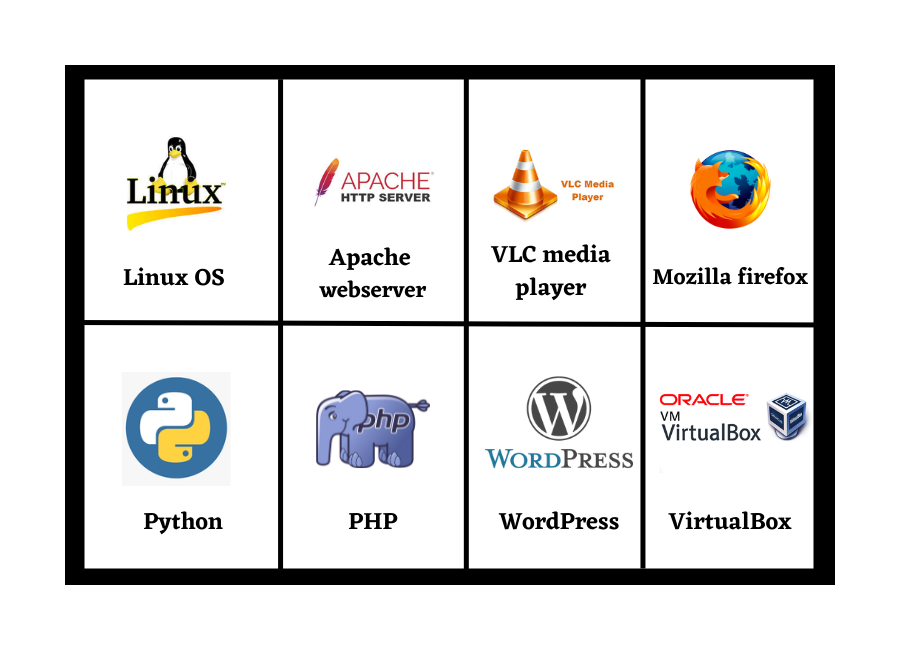
\includegraphics[scale=.4]{content/chapter1/images/opensource.png}
		\caption{Open Source Softwares}
		\label{fig:opensource1}
	\end{figure}
	
\end{flushleft}
\newpage
